\documentclass{report}
\usepackage[utf8]{inputenc}
\usepackage{amsfonts}
\usepackage{cite}
\usepackage{todonotes}
\usepackage{amsthm}
\usepackage{hyperref}
\usepackage{xcolor}
\usepackage[section]{placeins}

\newtheorem{theorem}{Theorem}

\title{Travelling salesman problem}
\author{Bastian Fredriksson \href{mailto:bastianf@kth.se}{bastianf@kth.se} \\ 
Fabian Ström \href{mailto:fabstr@kth.se}{fabstr@kth.se}}


\date{November 2015}

\begin{document}

\maketitle

\tableofcontents

\chapter{Introduction}
\section{Problem description}
\todo[inline]{Bastian.}
\todo[inline,backgroundcolor=green!25]{Fabian.}
The travelling salesman problem (TSP) is an optimization problem in computer science and operational research, and a special case of The Vehicle Routing Problem (VRP). The problem is to find the shortest Hamiltonian path in a undirected, weighted clique of size $n$. The variable $n$ is commonly called the number of \textit{cities} and instead of a path, we will talk about a \textit{tour}. The length of the tour is the sum $\sum_{i=1}^n{cost(i, j)}$ where $cost(i, j)$ is the cost of travelling between city $i$ and $j$.

For our particular problem $1 \le n \le 1000$, the cities are points $(x, y)$ in the plane, and $cost(i, j)=\left \lfloor{\sqrt{(x_1-x_2)^2+(y_1-y_2)^2} + 0.5}\right \rfloor$ (the Euclidean distance rounded to nearest integer). Note that due to cost function being rounded off, the triangle inequality does not hold for cities close to each other. For the rest of the paper, we will assume triangle inequality.

\section{Our approach}
\todo[inline]{Bastian.}
\todo[inline,backgroundcolor=green!25]{Fabian.} 
Our approach is to generate a set of solutions using the construction algorithms Nearest Neighbour, Nearest Insertion and MST heuristic. These algorithms were mainly selected because of their speed and simplicity. The solutions are improved using local search techniques and the best solution is picked. This makes it less probable to get a bad result from an algorithm underperforming for a certain set of cities.

For small problem instances, we will have time to examine a larger set of candidates. To ensure that each candidate is unique with high probability, our construction algorithms are randomized by use of PRNGs. Thus it is possible to invoke the same algorithm many times, and get a different candidate each time.

Inspiration for our implementation mainly stems from Extreme Algorithms\cite{extreme} and Heuristics for Traveling Salesman Problem.\cite{Nilsson}

\section{The tour object}
\todo[inline]{Bastian.}
\todo[inline,backgroundcolor=green!25]{Fabian.}
The tour object stores the tour as an array and supports the following methods:
\begin{enumerate}
\item \verb!print! Print the tour
\item \verb!swap! Swap two cities in the tour
\item \verb!index_of! Lookup the index of a city in constant time
\item \verb!transform! Transform the tour from an index-based to an order based representation
\item \verb!length! Measure the length of a tour
\item \verb!size! The number of cities in the tour
\item \verb!operator[]! Access the city number at the specified index
\end{enumerate}

The \verb!index_of! lookup is done quickly by maintaining an array which maps a city to its index in the tour. This speeds up our 2-Opt implementation \verb!opt2k! by a factor of $n$.%\todo{detta nämns inte i opt2?}.

For some algorithms, i.e nearest insertion and Clarke-Wright an index-based representation is more convenient than an order-based representation. However, other algorithms like 2-Opt require an order-based representation. An index-based representation is an array $A$ such that $A[i]$ contains the next city to visit after $i$ and an order-based representation is an array $A$ such that $A[i]$ contains the i:th city to visit.

The tour object support conversation between an index- and an order-based representation using \textit{transform()}.

\chapter{Algorithms used}
This chapter describes the algorithms used: Nearest Neighbour, Nearest Insertion, Minimum Spanning Tree and Clarke Wright. It also discusses 2-Opt which was used to improve the results.

\section{Nearest Neighbour}
\todo[inline]{Bastian.}
\todo[inline,backgroundcolor=green!25]{Fabian.}
The Nearest Neighbour algorithm is a simple greedy algorithm which picks a random city as the first city to visit. The next city in the tour is chosen as the city closest to the current city which has not yet been visited. The visited cities are stored in an unordered set for $O(1)$ lookup. This algorithm takes $O(n^2)$ time: At worst all possible next-city-candidates are checked and this is done once for each city.

During our testing, we found nearest neighbour to be significantly slower than e.g. nearest insertion which has the same worst-case running time. We believe this is due to cache misses.

\section{Nearest Insertion}
\todo[inline]{Bastian.}
This algorithm starts by defining a "triangle" of three random vertices $r_0$, $r_1$ and $r_2$ which forms the partial tour $r_0 \rightarrow r_1 \rightarrow r_2$. The rest of the vertices $x$ are included into the tour by selecting the edge (i, j) which minimises the quantity $cost(i, x) + cost(x, j) - cost(i, j)$. The running time of the algorithm is $O(n^2)$. There are other ways of selecting the initial tour. One way of doing it, which is slower, but probably more accurate is to calculate the convex hull and start insertion from there. However, since the solution will be improved using 2-Opt, we did not consider it worth implementing. 


\section{Minimum Spanning Tree}
\todo[inline]{Bastian.}
\todo[inline,backgroundcolor=green!25]{Fabian.}
The minimum spanning tree heuristic uses the traversal order of a minimum spanning tree of the graph to approximate the optimal solution within a factor of 2.

\begin{theorem}
$L \le 2L*$ where $L$ is the length of the solution produced by the MST heuristic and $L*$ is the optimal solution.  
\end{theorem}

\begin{proof}
Denote by $M$ the weight of the minimum spanning tree, i.e $\sum cost(i, j)$. First we observe that if we remove an edge from $L*$ we get a spanning tree. Thus $L* > M$. Next, consider traversing the tree in pre-order. Since each edge is traversed twice, the length of this tour will be $2M$. By combining with the previous inequality we get $2L* > 2M$ (the "pre-order tour" approximates within a factor of two). Finally we need to show that the tour taken by MST heuristic must be at most this long. Consider the situation below:
\begin{figure}[ht]
\centering
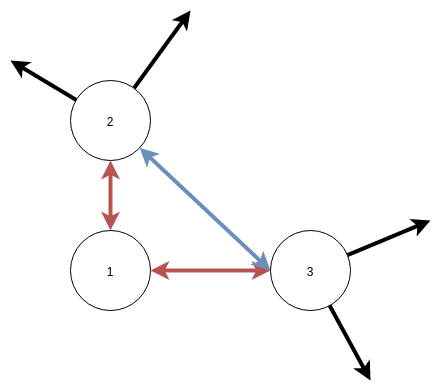
\includegraphics[width=60mm]{TriangleInequality}
\caption{An example of the triangle inequality. Taking the shortcut (blue edge) between 2 and 3 can never result in a longer tour then traversing the edges (1, 2) and (2, 3) marked in red.}
\end{figure}
Due to the triangle inequality, the tour produced by the MST heuristic must be shorter than the pre-order tour. Thus we have $2L* \ge L$.
\end{proof}

First a minimum spanning tree is created using Prim's algorithm. This step takes $O(n^2)$ time.

The MST heuristic is then traversing the tree in pre-order using DFS. The nice thing about the MST heuristic is that we can reuse the same MST to create many different tours quickly. Each new tour is created in linear time (since we only have to traverse each node once). 

The authors introduced randomization into the algorithm: Since it does not matter in which order the neighbours of a node is visited we shuffle the neighbour list before starting DFS. This means that the order in which the nodes are visited will (with high probability) be different for each traversal. The shuffling is done is linear time, so this does not impact the overall running time of the algorithm very much.

\section{Clarke-Wright}
\todo[inline]{Bastian.}
Clarke-Wright was developed for the VRP, but can be extended for the TSP as well. The first step is to select a random "hub vertex" $h$. The algorithm proceeds by for each pair of cities $(i, j)$ $i, j \neq h$ calculate a list of savings using the formula $cost(h, i) + cost(h, j) - cost(i, j)$. The final step is the construction of the tour: This is done by processing the list in descending order, inserting the first segment into the tour which does not violate the constraints 1) Each node in the tour must have a degree of at most two, and 2) no cycle must be created. 

The degree for each vertex is stored in an array which means that we can check constraint 1) in $O(1)$ time. Checking for cycles is done in $O(n)$ time, but this is only needed if the degrees of $i$ and $j$ are both 1 (this can be done in $O(1)$ time but was not implemented). The algorithm terminates when the number of nodes with a degree of two exceeds $n-2$. The last two segments $(i, h)$ and $(h, j)$ are inserted manually to complete the tour. The overall running time for the algorithm is $O(n^3)$, which is slower than the other heuristics. Due to a bug in our implementation, it is not shown in table of running times.

\section{2-Opt}
\todo[inline]{Bastian.}
\todo[inline,backgroundcolor=green!25]{Fabian.}
The local search technique used is 2-Opt. 2-Opt repeatedly picks a distinct pair of adjacent cities $(i,j)$ and $(a, b)$ such that replacing them with $(i, a)$ and $(j, b)$ makes the tour shorter, e.g if $cost(i, j) + cost(a,b) > cost(i,a) + cost(j, b)$. The problem with 2-Opt is the speed. The naive implementation \verb!opt2! looks at all $O(n^2)$ pairs of edges. To swap to edges, the subtour $j \rightarrow a$ must be reversed. If the tour is represented with an array, this takes $O(a-j)$ time, but it is only done once, which leaves us with $O(n^2)$ total running time for one iteration of 2-Opt. However, 2-Opt is usually repeated until no improvement can be found. Not much is known about the maximum number of iterations required to find a local minima, but is known to be bounded by $O(n^{10})$ for euclidean TSP where the cities are distributed at random in the $\mathbb{R}^2$.\cite{englert2006} Tours created by "smart" heuristics typically converge in linear time.

An optimization we implemented was to keep an array \verb!_index! which gives the index in the tour array for a a specific city $j$, thus eliminating the need to loop the array in linear time when the previous city $i$ in tour must be found (to determine the edge $(i, j)$).

\begin{figure}[ht]
\centering
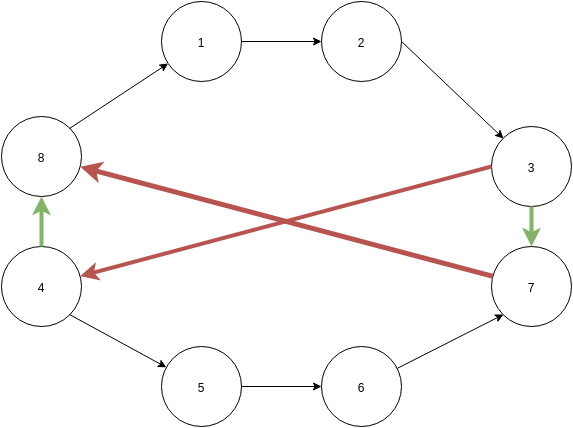
\includegraphics[width=80mm]{2-Opt}
\caption{A tour which can be improved using 2-Opt by replacing the edges (3, 4) and (7, 8) with (4, 8) and (3,7).}
\end{figure}

To speed up computations, one can use trees instead of arrays to store the tour, something we have not implemented. This makes it possible to swap a subtour in $O(log n)$. 

Another trick is to limit the search to the closest cities only (neighbourhood search) as described in "A case study of local Optimization"\cite{JohMcg97}. This will speed up the search, but yield less accurate results. The neighbour lists are calculated in a naive way by sorting, using $O(n^2\log n)$ time and $O(n^2)$ of space. This introduces some extra overhead, but its not a severe problem according to our benchmarks.

Our implementation \verb!opt2k! works as follows: We select a $k$ (typically $k=20$) and compute a neighbourhood list $L$ such that $L[i]$ contains the $k$ closest cities to $i$. To find candidates for $b$ we loop through $L$ in ascending order and pick $x$ if $cost(j, x) \ge cost(i, j)$. 

Another idea is to introduce a counter which counts the number of edges swapped. The algorithm is terminated when the counter exceeds a specific threshold value. This makes it possible to bound the running time of the algorithm from above, but requires the starting solution to be close to a local minima for 2-Opt to be accurate.

\section{3-Opt}
\todo[inline]{Bastian.}
\todo[inline,backgroundcolor=green!25]{Fabian.}
3-Opt selects three edges for removal and inserts them back again to make the tour shorter. Given the edges $(a, b)$, $(c, d)$ and $(e,f)$ where $a-f$ are indices, we identified the following 3-Opt tours: 

\begin{verbatim}
0 >>>> ad >>>> ec <<<< bf >>>> ~
0 >>>> ac <<<< be >>>> df >>>> ~
0 >>>> ae >>>> db >>>> cf >>>> ~
\end{verbatim}

The first tour results in the new edges $(a,b)$, $(c, d)$, $(e,f)$. \verb!0 >>>> a! means "take the tour from the first city to the a:th city in forward direction" and \verb!c <<<< b! means "take the tour from the c:th city to the b:th city in reverse direction". \verb!~! denotes the index of the last city in the tour.

Unfortunately, our 3-Opt implementation contained a bug, which meant that we could not use it on Kattis.

\begin{figure}[ht]
\centering
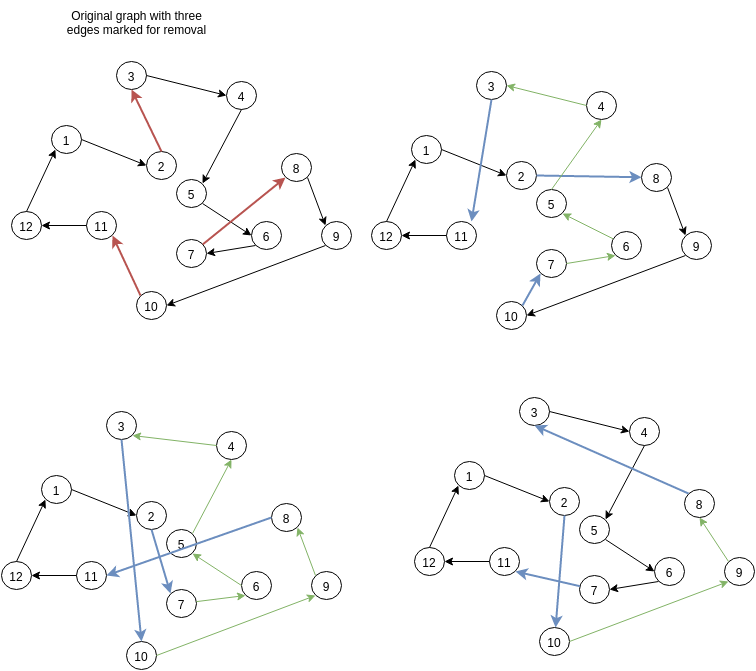
\includegraphics[angle=90,origin=c,width=140mm]{3-Opt}
\caption{Tour with three edges (in red) marked for removal by 3-Opt, and the three possible tours created from reinserting the edges (marked in blue). The edges marked in green are reversed.}
\end{figure}

\chapter{Experimental results and analysis}
\section{Kattis results}
Our best submission is 930972.

\section{A custom test case: A spiral}
\todo[inline]{Bastian.}
The illustrations were rendered with a special-built program created by the authors. The spiral shown in figure \ref{fig:spiral} was created using the following code.
\begin{verbatim}
output line "100"
for (t = 0; t < 50; t += 0.5) {
    x = 5t cos(t)
    y = 5t sin(t)
    output line x || " " || y 
}
\end{verbatim}

\begin{figure}[h!]
\centering
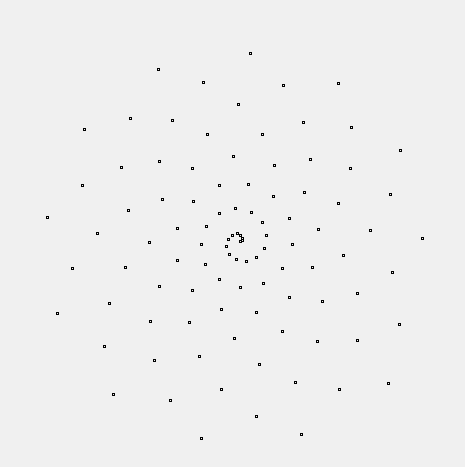
\includegraphics[width=80mm]{spiral}
\caption{A spiral of points.}
\label{fig:spiral}
\end{figure}

\begin{figure}[h!]
\centering
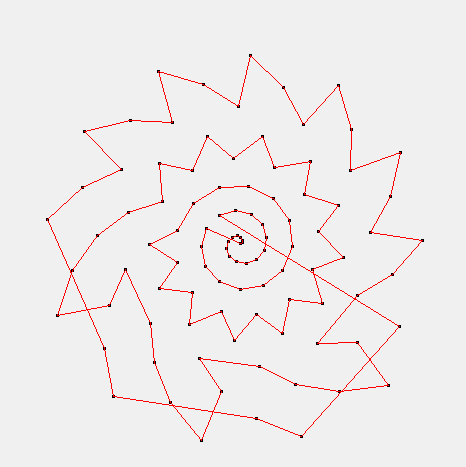
\includegraphics[width=80mm]{nn_spiral}
\caption{The solution created using nearest neighbour. Length 4389.}
\end{figure}

\begin{figure}[h!]
\centering
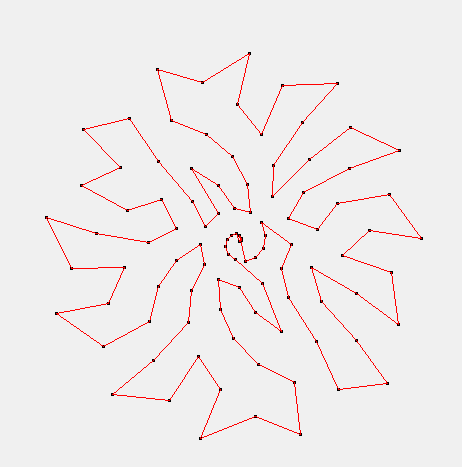
\includegraphics[width=80mm]{ni_spiral}
\caption{The solution created using nearest insertion. Length 4482.}
\end{figure}

\begin{figure}[h!]
\centering
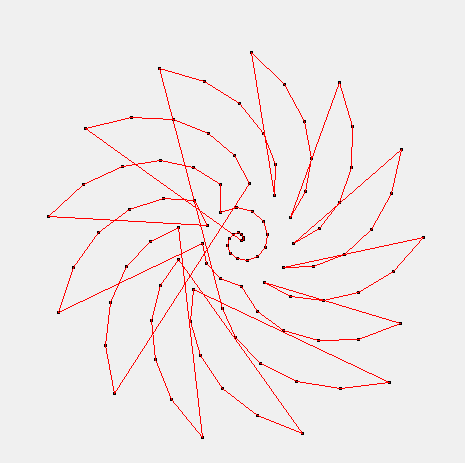
\includegraphics[width=80mm]{mst_spiral}
\caption{The solution created using MST heuristic. Length 6012.}
\end{figure}

\begin{figure}[h!]
\centering
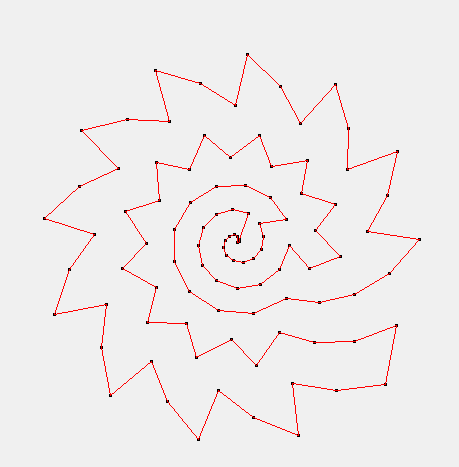
\includegraphics[width=80mm]{opt2_spiral}
\caption{A solution improved using 2-Opt. Length 4135.}
\end{figure}

\section{Random test cases}
\todo[inline,backgroundcolor=green!25]{Fabian.}
A lot of the testing was done on randomly generated test cases with $200$, $500$ and $1000$ nodes, the time distribution on how long different parts of the algorithm took can be seen in table~\ref{runningtimes}. Overhead refers to the work required to read input from \verb!stdin!, and the time it takes to construct the data structures used by the program. These data structures are the proximity list used by \verb!opt2k!, the distance matrix of precomputed cost values, and the minimum spanning tree used by MST heuristic.

A program was written to generate the random test cases.

Tables \ref{t200}, \ref{t500} and \ref{t1000} details how long the tour was for a random test case of size $200$, $500$ and $1000$ cities. 

    
%\begin{table}
%    \label{runningtimes}
%    \centering
%    \begin{tabular}{|l|l|l|l|}
%    \hline
%    ~                 & n=200 & n=500 & n=1000   \\ \hline
%    overhead          & 16   & 110  & 488        \\
%    nearest neighbour & 3.9  & 24   & 97         \\
%    nearest insertion & 0.2  & 1.1  & 8.2        \\
%    mst-heuristic     & 0.1  & 0.35 & 0.69       \\
%    2-opt             & 21   & 356  & $>$ 2000   \\
%    2-opt k=200       & 18 p  & 4910 & 117        \\
%    2-opt k=100       & 5    & 10   & 36         \\
%    2-opt k=40        & 1.1  & 2.5  & 9.8        \\
%    2-opt k=20        & 0.31 & 0.85 & 2.4        \\
%    2-opt k=10        & 0.14 & 0.32 & 0.9        \\ \hline
%    \end{tabular}
%    \caption{Running time in milli seconds for different parts of the algorithm}
%\end{table}

\begin{table}
  \centering
  \begin{tabular}{|l|l|l|l|l|l|l|l|l|l|l|} \hline
size & nn    & ni     & mst    & opt2 & k=200 & k=100 & k=40 & k=20 & k=10 \\ \hline
200  &       3.94     & 0.1647 & 0.1504 & 28.71 & 64.56 & 22.34 & 6.028 & 2.058 & 0.4138\\ \hline 
500  &       24.49    & 1.319  & 0.368 & 353.8 & 286.3 & 98.17 & 26.7 & 5.31 & 1.119\\ \hline 
1000 &       97.11    & 8.197  & 0.7051 & 2997 & 958.8 & 435.8 & 83.54 & 14.39 & 2.85\\ \hline
  \end{tabular}
  \caption{Running time in milliseconds for different parts of the algorithm (as a mean of 10 samples, opt2 and variants were performed on the nearest neighbour version). In the k=$x$ columns the $k$ closest cities were looked at instead of all).}
  \label{runningtimes}
\end{table}

\begin{table}
  \centering
  \begin{tabular}{|l|l|l|l|l|l|l|l|}
    \hline
   &    unimproved      & opt2         & opt2, k=200  & opt2, k=100  & opt2, k=40   & opt2, k=20   & opt2, k=10  \\ \hline
nn & 7141 & 5649 & 5872 & 6040 & 6362 & 6745 & 6817 \\ \hline
ni & 6102 & 5957 & 5999 & 6032 & 6083 & 6093 & 6102 \\ \hline
mst & 7432 & 5841 & 5965 & d6163 & 6648 & 7031 & 7342 \\ \hline
  \end{tabular}
  \caption{Length of tour, random test case with 200 cities (all lengths are presented as a mean of 10 samples).}
  \label{t200}
\end{table}


\begin{table}
  \centering
  \begin{tabular}{|l|l|l|l|l|l|l|l|}
    \hline
   &    unimproved      & opt2         & opt2, k=199  & opt2, k=100  & opt2, k=40   & opt2, k=20   & opt2, k=10  \\ \hline
nn & 10559 & 8962.1 & 9321.1 & 9472.7 & 10006 & 10288 & 10456 \\ \hline
ni & 9437.5 & 9165.6 & 9379.6 & 9413.6 & 9425.1 & 9434.2 & 9437.2 \\ \hline
mst & 11964 & 9194.1 & 9723.7 & 10264 & 11015 & 11789 & 11885 \\ \hline
  \end{tabular}
  \caption{Length of tour, random test case with 500 cities (all lengths are presented as a mean of 10 samples).}
  \label{t500}
\end{table}


\begin{table}
  \centering
  \begin{tabular}{|l|l|l|l|l|l|l|l|}
    \hline
   & unimproved      & opt2         & opt2, k=200  & opt2, k=100  & opt2, k=40   & opt2, k=20   & opt2, k=10  \\ \hline
nn & 13970 & 12210 & 12764 & 13100 & 13587 & 13796 & 13911 \\ \hline
ni & 12966 & 12541 & 12947 & 12951 & 12963 & 12965 & 12966 \\ \hline
mst & 16097 & 12520 & 13657 & 14313 & 15412 & 15903 & 16055 \\ \hline
  \end{tabular}
  \caption{Length of tour, random test case with 1000 cities (all lengths are presented as a mean of 10 samples).}
  \label{t1000}
\end{table}

\section{Analysis}
\todo[inline,backgroundcolor=green!25]{Fabian.}
For the spiral Nearest Neighbour and Nearest Insertion gave pretty good results without any improvement, though it could be improved a little by using 2-Opt. Looking at the pictures nearest insertion and MST Heuristic seems to favour going from the center to the edge and back, whilst Nearest Neighbour and the tour improved using 2-Opt follows the expected spiral.

Our tests indicates that for random test cases the best result is obtained by running 2-Opt on a tour given by the Nearest Neighbour algorithm though this result comes at a cost: together with 2-Opt, Nearest Neighbour is multiple orders of magnitude slower than Nearest Insertion and MST Heuristic. It is worth noting that an unimproved Nearest Insertion seems to be not very far from the best Nearest Neighbour with 2-Opt result while being a lot faster.

On Kattis, results improved as expected, if the number of candidate solutions was increased. For large test cases, we got better results when using our naive 2-Opt implementation on only one candidate solution, rather than generating a lot of candidate solutions, and using the faster 2-Opt implementation \verb!opt2k!. 

\bibliographystyle{acm}
\bibliography{refs}
\addcontentsline{toc}{chapter}{Bibliography}





\end{document}